\section{Uranerz}

\subsection{Gammaspektrum}

In diesem Versuchsteil wollen wir ermitteln, welche Elemente wir anhand des Gammaspektrums des Uranerzes in diesem nachweisen können. Dazu haben 
wir haben das Uranerz eine Stunde auf unserem Ge-Detektor gestellt, um auch die schwächeren Linien über das Rauschen zu heben.\\
In der daraus entstehenden Abbildung \ref{Uranerz} kann man deutlich die charakteristischen Linien herrauslesen und zuzuordnen\footnotemark.
\footnotetext{\url{https://de.wikipedia.org/wiki/Gammaspektroskopie}, Eingesehen am 15.09.2021}

\begin{figure}[h]
    \centering
    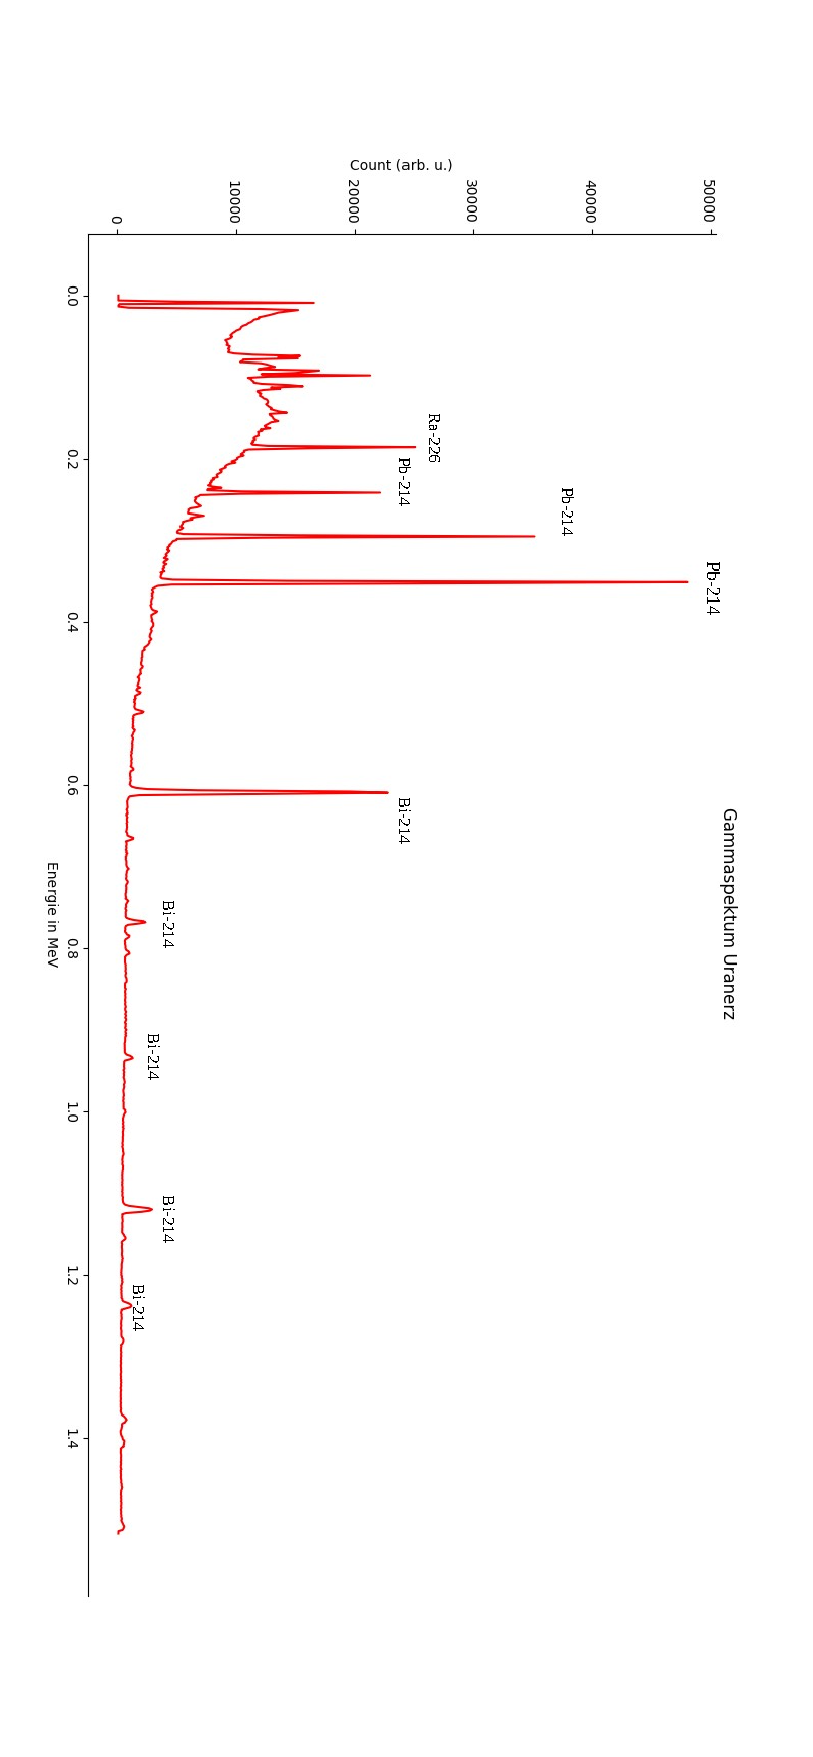
\includegraphics[width = 11cm]{Bilder/Auswertung/UranerzSpektrum.pdf}
    \caption{Spektrum des Uranerz. Zu den Zerfällen gehörende Elemente sind zugeordnet. Manche Peaks im unteren Spektralbereich waren nicht identifizierbar}
    \label{Uranerz}
\end{figure}

\clearpage
\subsection{Massenabsorptionskoeffizient}

Nun wiederholen wir die Messung aus Kapitel \ref{section:Absorbtionskoeff} mit Blei. Dabei haben wir diesmal den Vorteil, dass wir aufgrund der vielen 
Spektrallinien die Energieabhängigkeit des Massenabsorptionskoeffizient beobachten können. Dafür haben wir eine leere Messung, eine Messung mit 1,2,3,4 und 7 Bleiplatten mit 
jeweils einem Millimeter zu Verfügung. Die Absorptionskoeffizienten werden exemplarisch an drei Linien berechnet. 
Dafür verwenden wir drei sehr deutlich sichtbare Linien:
\begin{center}
    \centering
    \begin{tabular}{lr}
        Ra-226 & (0,185 $\pm$ 0,003)\,MeV\\
        Pb-214 & (0,351$\pm$ 0,003)\,MeV\\
        Bi-214 & (0,609$\pm$ 0,003)\,MeV\\
    \end{tabular}
\end{center}

Nach dem Berechnen der Massenabsorptionskoeffizienten kommen wir auf folgende Werte.


\begin{center}
    \centering
    \textcolor{red}{$\frac{\mu_{0,185MeV}}{\rho_{Pb}} = (0,3\pm0,2) \mathrm{cm}^{2} \mathrm{g}^{-1}$}\\
    \textcolor{red}{$\frac{\mu_{0,351MeV}}{\rho_{Pb}}= (0,17\pm0,03) \mathrm{cm}^{2} \mathrm{g}^{-1}$}\\
    \textcolor{red}{$\frac{\mu_{0,609MeV}}{\rho_{Pb}}= (0,141\pm0,004) \mathrm{cm}^{2} \mathrm{g}^{-1}$}\\
\end{center}

Man sieht sehr deutlich, dass der Absorptionskoeffizient stark von der Energie des einfallenden Teilchens abhängt. Wenn man den Zusammenhang plottet, wie in Abbildung \ref{AbsEne}, dann meint man 
einen exponentiellen Zusammenhang zu erkennen.

\begin{figure}
    \centering
    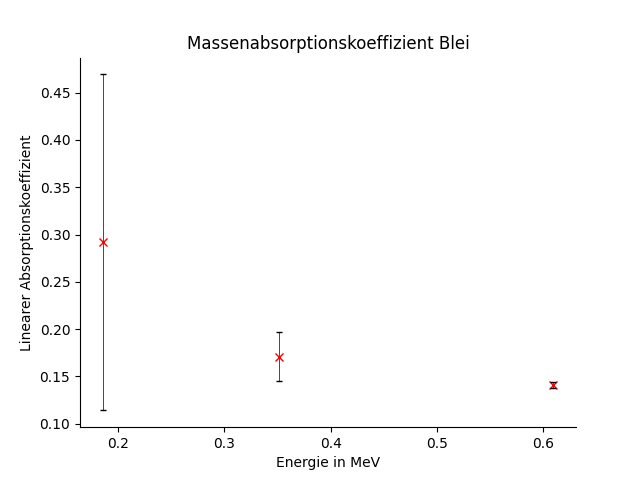
\includegraphics[width = 12cm]{Bilder/Auswertung/AbsorbtionBleiEnergie.png}
    \caption{Energieabhängigkeit des Absorptionskoeffizienten}
    \label{AbsEne}
\end{figure}

Dieser ist auch näherungsweise vorhanden, da, wenn man den Verlauf des Absorptionskoeffizienten nachschaut, man in unserem Bereich einen 
exponentiellen Zusammenhang sieht (die y-Werte in Abbildung \ref{AbsLit} sind logarithmisch angetragen). Dieser sollte dort auch vorhanden sein, da 
wir unterhalb der in Abbildung \ref{AbsLit} gezeigten Absorptionskante sind.


\begin{figure}
    \captionsetup{justification=centering,margin=2cm}
    \centering
    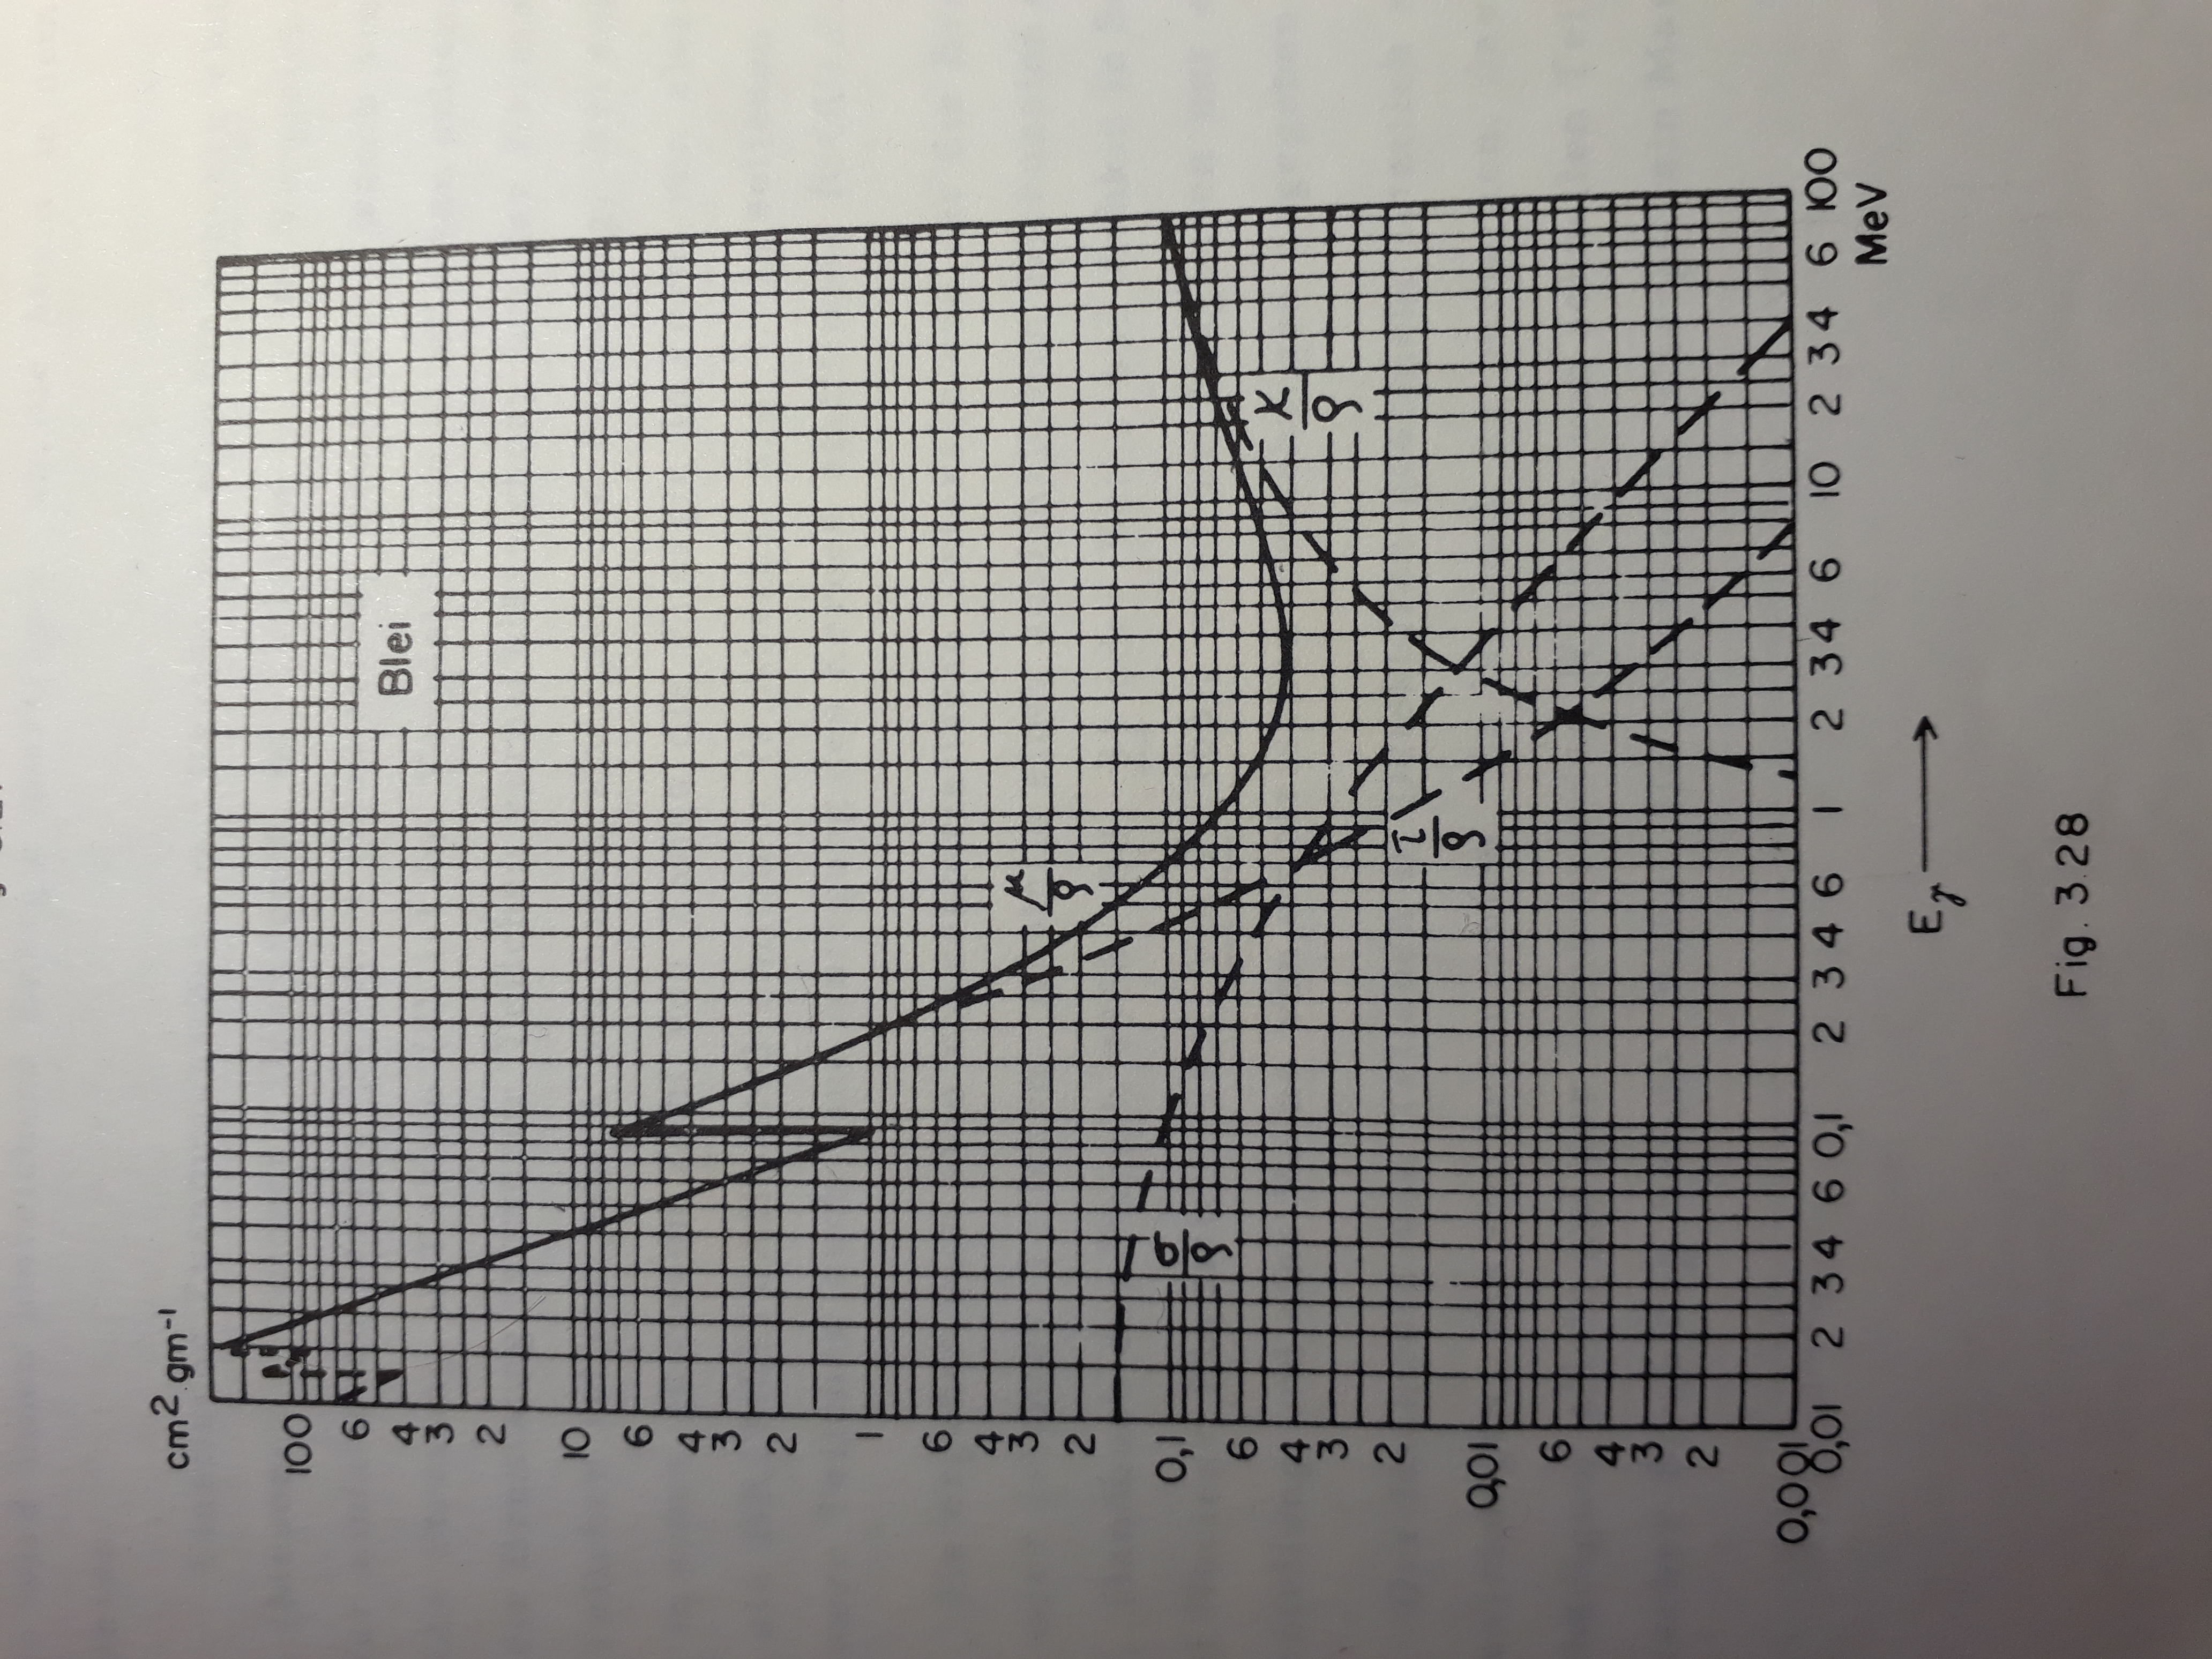
\includegraphics[width = 12cm, angle = -90]{Bilder/Auswertung/AbsMamier.jpg}
    \caption{Energieabhängigkeit des Absorptionskoeffizienten laut Literatur \cite[S.46a]{Marmier1977}}
    \label{AbsLit}
    
\end{figure}
